\documentclass[preprint,12pt,authoryear]{elsarticle}
\makeatletter
\def\ps@pprintTitle{%
	\let\@oddhead\@empty
	\let\@evenhead\@empty
	\def\@oddfoot{\centerline{\thepage}}%
	\let\@evenfoot\@oddfoot}
\makeatother
\usepackage{booktabs}
\usepackage{subfigure, epsfig, epstopdf}
\usepackage{graphicx}
\usepackage{amsmath}
\usepackage{mathrsfs}
\usepackage{amssymb}
\usepackage{multirow, multicol}
\usepackage{color}
\usepackage{soul}
\usepackage{setspace}
\usepackage[left=0.8in,top=1in,right=0.8in,bottom=1in, nohead]{geometry}
\usepackage[colorlinks=true,backref=true,hyperindex,citecolor=blue,linkcolor=blue]{hyperref}
\usepackage{natbib}
\usepackage{tabularx}
\usepackage{colortbl}
\usepackage{titlesec}
\usepackage{enumerate}
\usepackage{amsfonts}
\usepackage{threeparttable}
\usepackage{float}
\usepackage{url}
\usepackage{hyperref}
\usepackage[titletoc,title]{appendix}
\usepackage{booktabs}
\usepackage{csvsimple}

\titleformat{\paragraph}[block]{\normalsize\bfseries}{\theparagraph}{1em}{}

\bibpunct{(}{)}{;}{a}{,}{,}


\newtheorem{theorem}{Theorem}
\newtheorem{lemma}{Lemma}
\newtheorem{proposition}{Proposition}
\newtheorem{corollary}[theorem]{Corollary}
\newtheorem{assumption}{Assumption}

\newenvironment{proof}{\paragraph{Proof.}}{\hfill$\square$}
\newenvironment{definition}[1][Definition]{\begin{trivlist}
		\item[\hskip \labelsep {\bfseries #1}]}{\end{trivlist}}
\newenvironment{example}[1][Example]{\begin{trivlist}
		\item[\hskip \labelsep {\bfseries #1}]}{\end{trivlist}}
\newenvironment{remark}[1][Remark]{\begin{trivlist}
		\item[\hskip \labelsep {\bfseries #1}]}{\end{trivlist}}
\newenvironment{mydescription}{\begin{description}
		\setlength{\itemsep}{0pt}\setlength{\parskip}{0pt}\setlength{\parsep}{0pt}}{\end{description}} 

\newcommand{\bI}{\mathcal I}
\newcommand{\bN}{\mathcal N}
\newcommand{\bE}{\mathbb E}
\newcommand{\bR}{\mathfrak R}
\newcommand{\bQ}{\mathbb Q}
\newcommand{\bF}{\mathbb F}
\newcommand{\bP}{\mathbb P}
\newcommand{\by}{\mathbf y}
\newcommand{\bX}{\mathbf X}
\newcommand{\bT}{\mathbf T}
\newcommand{\bD}{\mathbf D}
\newcommand{\bt}{\mathbf t}
\newcommand{\bx}{\mathbf x}
\newcommand{\bs}{\mathbf s}
\newcommand{\bU}{\mathcal U}
\newcommand{\bW}{\mathcal W}
\newcommand{\pr}{\textup{Pr}}


\newcommand{\mb}[1]{\mbox{\boldmath \ensuremath{#1}}}
\renewcommand{\vec}[1]{\boldsymbol{#1}} 
\newcommand{\vectilde}[1]{\tilde{\boldsymbol{\boldsymbol{#1}}}}
\newcommand{\tildevarepsilon}{\tilde{\varepsilon}}
\newcommand{\vecvarepsilon}{\vec{\varepsilon}}
\newcommand{\vectildevarepsilon}{\tilde{\vec{\varepsilon}}}
\newcommand{\vectau}{\vec{\tau}}
\newcommand{\vecalpha}{\vec{\alpha}}
\doublespacing
\graphicspath{{imgs/}} 


\begin{document}
\setlength{\abovedisplayskip}{3pt}
\setlength{\belowdisplayskip}{3pt}

\begin{titlepage}
    \begin{center}
        \vspace*{1cm}
        
        \Huge
	 \textbf{Optimal design of decentralized constructed wetland treatment system under uncertainties}\\        
	 \noindent\makebox[\linewidth]{\rule{0.7\paperwidth}{0.4pt}}
        \vspace{0.5cm}
        \LARGE
        IE4100 Progress Report
        
        \vspace{1.5cm}
        
        Yeow Li Teng Cheryl\\
	  A0116781A\\
	  Mentor: A/P Ng Tsan Sheng, Adam
        
        \vfill
        
%        A thesis presented for the degree of\\
%        Doctor of Philosophy
        
        \vspace{0.8cm}
        
%        \includegraphics[width=0.4\textwidth]{university}
        
        \Large
        Department of Industrial \& Systems Engineering\\
        National University of Singapore\\
%        Country\\
%        Date
        
    \end{center}
\end{titlepage}

%\begin{frontmatter}
	

	
%	  \title{\textbf{Optimal design of decentralized constructed wetland treatment system under uncertainties}}

%\begin{abstract}

%\end{abstract}

%\begin{keyword}

%\end{keyword}
%\end{frontmatter}



 
\section{Model}
A basic list of model parameters and decision variables is provided in Table \ref{table:modelparameter}. Other notations would be introduced and defined as per required in the rest of the paper. 

\begin{table}[!htpb]
	\setlength{\extrarowheight}{1.5mm}
	\caption{Notations of model parameters and decision variables}
	\begin{tabular}{|p{1.5cm} p{16cm}|}
		\hline
		\multicolumn{2}{|c|}{Indices} \\
		\hline
		$i$ & index of wastewater sources, $i\in\{1,2,...,I\}$\\
		$j$ & index of potential CW locations, $j\in\{1,2,...,J\}$ \\
		$m$ & index of evaluated water pollutants, $m\in\{1,2,...,M\}$\\
		$k$ & index of CW construction options, $k\in\{0,1,2,...,K\}$\\
		\hline
		\multicolumn{2}{|c|}{Model parameters} \\
		\hline
		$\varepsilon_i^m$ & concentration of pollutant $m$ in the wastewater source $i$ (mg/m$^3$)\\
		$\varepsilon_{in,j}^m$ & concentration of pollutant $m$ in the influent of CW site $j$ (mg/m$^3$)\\
		$\varepsilon_{out,j}^m$ & concentration of pollutant $m$ in the effluent of CW site $j$ (mg/m$^3$)\\
		$C_{j}^{m*}$ & background concentration of pollutant in the wastewater at CW site $j$ (mg/m$^3$)\\
		$\tau_{j}^{m}$ & treatment target for pollutant $m$ in CW site $j$ (mg/m$^3$)\\
		$F_{i}$ & total wastewater flow generated by source $i$ (m$^3$/d)\\
		$Q_{jk}$ &  flow capacity of CW in option $k$ for site $j$ (m$^3$/d)\\
		$A_{jk}$ & area of CW in option $k$ for site $j$ (m$^2$)\\
		$c_{cw,jk}$ & construction cost of CW in design option $k$ for site $j$ (\$) \\	
		$d_{ij}$ & distance between wastewater source $i$ and site $j$ (m)\\
		$c_s$ & unit construction cost of sewer lines per distance (\$/m)\\
		\hline
		\multicolumn{2}{|c|}{Decision variables}\\
		\hline	
		$x_{ij}$ & binary variable, $x_{ij}=1$ if sewer lines are constructed from wastewater source $i$ to CW site $j$ and $0$ otherwise\\
		$y_{jk}$ & binary variable, $y_{jk}=1$ if construction option $k$ is chosen for site $j$ and $0$ otherwise. In particular, $z_{j0}$ denotes the choice of not constructing any CWs in site $j$\\
		$z_{ij}$ & $0$ $\leq$ $z_{ij}$ $\leq$ $1$, proportion of wastewater flow assigned from wastewater source $i$ to the CW in site $j$ \\
		\hline	
	\end{tabular}

	\label{table:modelparameter}
\end{table}

Before the uncertainty component is addressed, we may come up with a deterministic model to solve the problem first. The objective of the problem is to minimize the total cost of implementing the system in a region. The following constraints formulate the constructed wetlands construction option, wastewater allocation between sources and constructed wetlands, pollutant removal performance, treatment target fulfillment:

\textbf{Constructed wetlands design options:} Let $z_{jk}$ be a binary variable that describes the design option $k$ selected for the constructed wetlands site $j$. In the case where $k=0$, there will be no constructed wetlands on the potential site $j$. Otherwise, any other values for $k$ will correspond to the respective design options available. When $z_{jk} = 1$, it means that there will be a constructed wetlands of type $k$ at site $j$. The different design options result in different construction costs and pollutant removal capacities. To maintain the logic of the problem, only one design option can be selected at each site. Hence, the following constraint is introduced:
\begin{equation*}
	\begin{split}
	&\sum_{k=0}^{K}z_{jk}=1,~~~\forall j\\
	&z_{jk}\in\{0,1\},~~~\forall j,k
	\end{split}
\end{equation*}

\textbf{Wastewater allocation from sources to sites:} Let $y_{ij}$ be a binary variable that describes the interconnection between the wastewater source $i$ and potential contructed wetlands site $j$. When $y_{ij} = 1$, wastewater is allowed to flow from source $i$ to site $j$. Otherwise, $y_{ij} = 0$. To ensure that the wastewater is allocated consistently, the total of all the flows from a single source $i$ should be equal to the flow generated by source $i$. On top of that, the total volume of wastewater flowing into a constructed wetland cannot exceed the design capacity of the constructed wetland. Finally, there should only be wastewater sent to a site if there is a connection ($y_{ij} = 1$). If $x_{ij}$ represents the proportion of wastewater sent from source $i$ to site $j$, $F_{i}$ is the total wastewater flow from source $i$ and $Q_{jk}$ is the maximum flow capacity accepted by site $j$ with design option $k$:
\begin{alignat*}{2}
    &\sum_{i=1}^{I}x_{ij}F_{i}\leq \sum_{k=0}^{K}Q_{jk}z_{jk},~~ &&\forall j\label{eq:CWcapacity}\\
	&\sum_{j=1}^{J}x_{ij}=1, &&\forall i \nonumber\\
	&0 \leq F_ix_{ij}\leq F_iy_{ij},&&\forall i,j\nonumber\\
	& y_{ij}\in\{0,1\}&&\forall i,j\nonumber
\end{alignat*}
\textbf{Pollutant removal performance and treatment target fulfillment:} First, we consider the influent of the constructed wetlands. The water that is entering the constructed wetlands should have the same amount of pollutants as all of the sources that are contributing wastewater to the site. To determine the pollutant concentration in the effluent, we use a first-order $k-C^*$ model \citep{rousseau2004model} to calculate the pollutant removal. Finally, to ensure that treatment targets are met, the effluent pollutant concentrations should be subject to treatment target constraints. 
\begin{alignat*}{2}
	&{\sum_{i=1}^{I}F_{i}y_{ij}\varepsilon_{i}^{m}} = \varepsilon_{in,j}^{m}{\sum_{i=1}^{I}F_{i}y_{ij}} &&\forall j,m\\
	&[\varepsilon_{in,j}^{m}-{c}_{j}^{m*}]\sum_{k=0}^{K}e^{-\frac{A_{jk}}{Q_{jk}}k_{A}^{m}}z_{jk}+c_{j}^{m*} = \varepsilon_{out,j}^{m} &&\forall j,m\\
	&\varepsilon_{out,j}^{m}\leq \tau_{j}^{m}~~~&&\forall j\\
\end{alignat*}
%The following deterministic model is developed from the above constraints. It is a \emph{Mixed-Integer Linear Programming} (MILP) problem (Model D):
\newpage
\begin{equation*}\label{modelD}
\begin{aligned}
	\text{Model D}:~~&min \sum_{i=1}^{I}\sum_{j=1}^{J}d_{ij}c_s x_{ij} + \sum_{j=1}^{J}\sum_{k=1}^{K}c_{cw,jk}y_{jk}\\~~
	\mbox{s.t.}~~
	&\sum_{i=1}^{I} [ e^{-\frac{A_{jk}}{Q_{jk}}k_{A}^{m}} \varepsilon_i^m - e^{-\frac{A_{jk}}{Q_{jk}}k_{A}^{m}} C_j^{m*} - (\tau_j^m - C_j^{m*})] z_{ij} - M(1 - y_{jk}) \leq 0 && \forall j,k,m\\
 	&\sum_{i=1}^{I} z_{ij} \leq \sum_{k=0}^K Q_{jk} y_{jk} && \forall j\\
	&\sum_{j=1}^J z_{ij} = F_i && \forall i\\
	&z_{ij} \leq F_i x_{ij} && \forall i,j\\
	&x_{ij} + y_{j0} <= 1 && \forall i,j\\
	&\sum_{k=0}^{K}y_{jk} = 1&&\forall j\\
	&x_{ij} \in \{0,1\}&&\forall i,j\\
	&y_{jk} \in \{0,1\}&&\forall j,k\\
	&z_{ij} \geq 0&&\forall i,j\\
%	&{\sum_{i=1}^{I}F_{i}\varepsilon_{i}^{m}x_{ij}} = {\sum_{i=1}^{I}F_{i}\varepsilon_{i}^{m}}&&\forall j,m\\
%	&\sum_{k=1}^{K} c_{j}^{m*} e^{-\frac{A_{jk}}{Q_{jk}}k_{A}^{m}} z_{jk} + \sum_{i=1}^{I}\sum_{k=1}^{K} \varepsilon_i^m s_{ijk} \leq \tau_j^m - c_j^{m*} && \forall j,m\\
%	&x_{ij} + z_{jk} - s_{ijk} \leq 1 && \forall i, j, k\\
%	&s_{ijk} - x_{ij} \leq 0 && \forall i, j, k\\
%	&s_{ijk} - z_{jk} \leq 0 && \forall i, j, k\\
%	&[\varepsilon_{in,j}^{m}-{c}_{j}^{m*}]\sum_{k=0}^{K}e^{-\frac{A_{jk}}{Q_{jk}}k_{A}^{m}}z_{jk}+c_{j}^{m*} \leq \tau_{j}^{m}&&\forall j,m\\
%	&\sum_{i=1}^{I}F_{i}x_{ij}\leq\sum_{k = 0}^{K}Q_{jk}z_{jk}&&\forall j\\
%	&\sum_{j=1}^{J}x_{ij} = 1&&\forall i\\
%	&\sum_{k=0}^{K}z_{jk} = 1&&\forall j\\
%	&x_{ij}\leq y_{ij}&&\forall i,j\\
%	&y_{ij} \in \{0,1\}&&\forall i,j\\
%	&z_{jk} \in \{0,1\}&&\forall j,k\\
%	&0 \leq x_{ij} \leq 1&&\forall i,j\\
%	&0 \leq s_{ijk} \leq 1&&\forall i,j,k\\
\end{aligned}
\end{equation*}
\newpage
\subsection{Case study: a decentralized CWs system for municipal wastewater treatment}
\subsubsection{Mobile, Alabama}
With 412,992 people, Mobile County is the second most populated county within the state Alabama in the United States. The population of Mobile County has been steadily increasing \citep{uscb2002census}. As populations grow, several fringe communities are created. To manage the wastewater produced by such communities, the traditional approach is to link these fringe communities up with long length large diameter pipes to transport all the wastewater to a single municipal wastewater treatment plant to be processed and then released into nearby water sources. The Mobile Area Water \& Sewer System (MAWSS) serves approximately 530 square kilometres in Mobile County \citep{mawss2015}, mostly through centralised wastewater treatment facilities. However, annual operations and maintenance costs for such centralised wastewater management systems have been shown to be costlier than decentralised ones, where the wastewater is processed and released within the community \citep{mawss2015}. Thus, implementation of decentralised wastewater management systems such as constructed wetlands are being considered to manage costs in the long term. 

\subsubsection{Data Collection}
\textbf{Case Study Area:}\begin{figure}[!b]
	\centering
	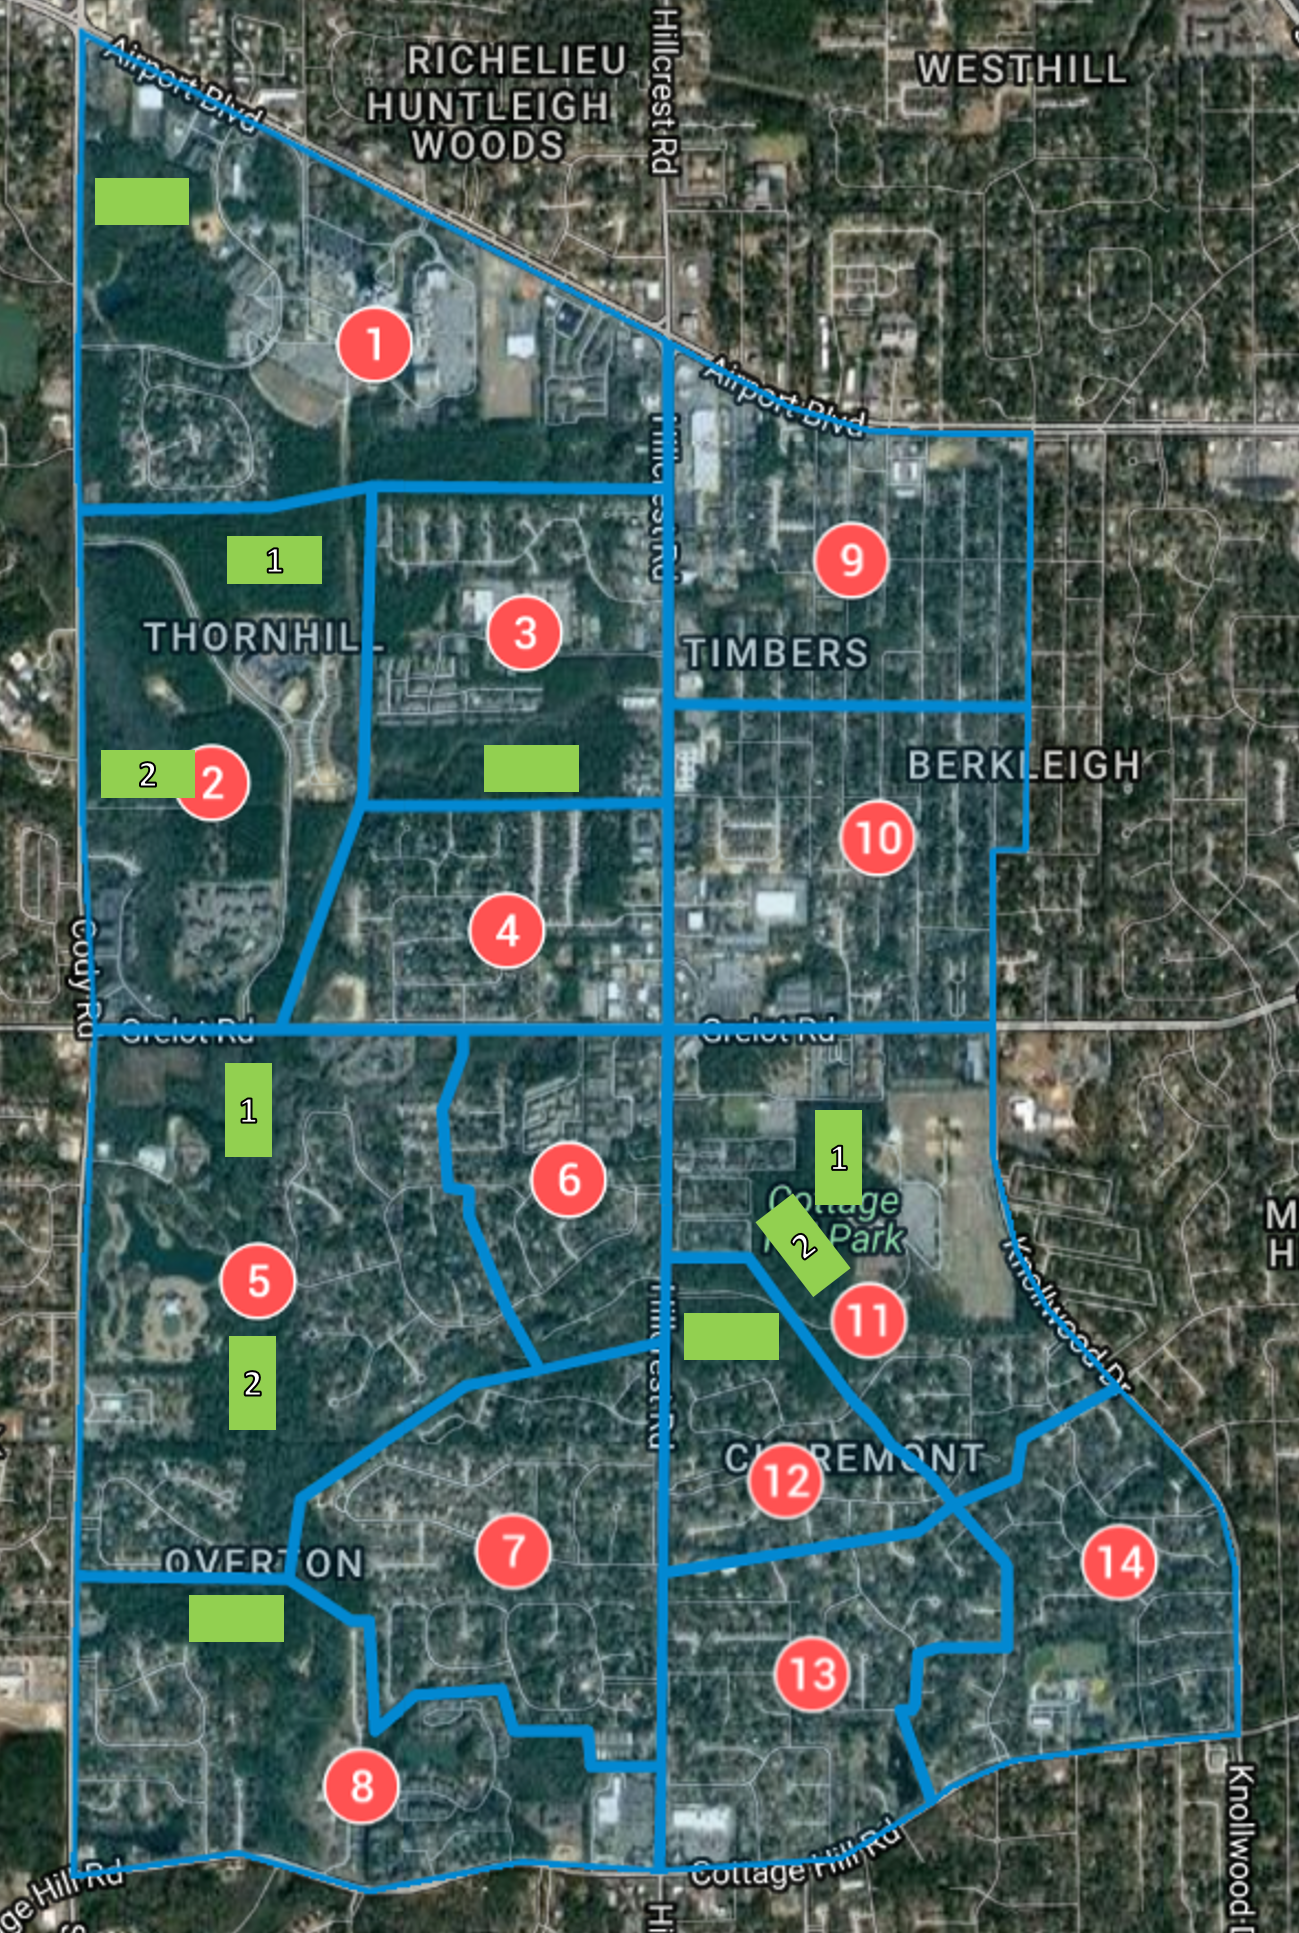
\includegraphics[width=0.35\textwidth]{blocks.png}
	\caption{Case study area in Mobile, Alabama.}
	\label{fig:blocks}
\end{figure}
The site chosen for the case study is near Mobile Regional Airport. It is a suburban area, mostly consisting of residences. As the objective of the project is to show how the optimization model can be applied, we have chosen a smaller area to keep the computation resources required reasonable. Hence, the site has been divided into 14 blocks based on six census tract blocks. The blocks are represented with blue outlines in Fig. \ref{fig:blocks}. Geographic information about the region listed in Table \ref{table:geodata} was also retrieved from the census. \citep{acs2015} For each block, we have assumed a point source for the wastewater (see red circles).

Potential sites for the constructed wetlands were identified from Google Maps and represented in Fig. \ref{fig:blocks} as green rectangles. These areas are empty and thus the construction of wetlands there will impact few residents negatively. A point location is used to represent each of these sites. The coordinates of the potential sites are stated in Table \ref{table:cwdata}. The distances between the wastewater sources and potential sites were calculated as well and stated in Table \ref{table:distdata}. 

\textbf{Pollutants:} Once again, to keep the model manageable, we have narrowed down the number of pollutants to three, as seen in Table \ref{table:polldata}. The pollutants have been selected based on the effects of pollution if these substances were not removed. In this case study, we will set the treatment target to be the same regardless of the intended use for the treated water.

\textbf{Design options:} We have determined four design options for the constructed wetlands and their respective construction costs can be found in Table \ref{table:ccwdata}. The formula for estimating the cost can be found in \cite{kadlec2009}.

\textbf{Sewer pipe construction cost:} Based on \cite{kadlec2009}, the normal size of sewer pipes for treatment wetlands vary from $10-30 cm$ diameter pipes. Hence, the sewer pipe construction cost is estimated to be about $US\$134/m$ \citep{usepa2000} after revising to latest prices. \\

The above information provides a good set-up to determine optimal locations for constructed wetlands to be built within Mobile, Alabama. 

\section{Further Directions}
Proceeding from here, the next step would be to find a solution for the deterministic model, which will be done using MATLAB. After which, work will commence on developing the probabilistic model and running it. 


%\section{Conclusions}
\newpage
\section*{Appendix}\label{Chap:appendix}

\begin{table}[!h]
	\caption{Geographical information about the 14 blocks.}
	\label{table:geodata}
	\centering
	\begin{tabular}{c c c c c c}
		\csvautotabular{data/blockgeo.csv}
	\end{tabular}
\end{table}

\begin{table}[!h]
	\caption{Coordinates of the potential constructed wetlands sites.}
	\label{table:cwdata}
	\centering
	\begin{tabular}{ c c c }
		\csvautotabular{data/cwgeo.csv}
	\end{tabular}
\end{table}

\begin{table}[!h]
	\caption{Distance in $km$ between the wastewater sources and potential constructed wetlands sites.}
	\label{table:distdata}
	\centering
	\begin{tabular}{ c c c c c c c c c c c c}
		\csvautotabular{data/dist.csv}
	\end{tabular}
\end{table}

\begin{table}[!h]
	\caption{Selected pollutants with the respective indicators coupled with average pollutant concentration in the wastewater source and the treatment targets.}
	\label{table:polldata}
	\centering
	\makebox[\linewidth]{
	\begin{tabular}{c c c c c}
		\csvautotabular{data/pollutants.csv}
	\end{tabular}
	}
\end{table}

\begin{table}[!h]
	\caption{Construction cost of constructed wetlands with four different design options as well as projected area and flow capacity.}
	\label{table:ccwdata}
	\centering
	\begin{tabular}{c c c c}
		\csvautotabular{data/ccw.csv}
	\end{tabular}
\end{table}

\addcontentsline{toc}{chapter}{Appendix}
\setcounter{equation}{0}
\renewcommand{\theequation}{A.\arabic{equation}}
\setcounter{figure}{0}
\renewcommand{\thefigure}{A.\arabic{figure}}
\setcounter{section}{0}
\renewcommand{\thesection}{A-\arabic{section}}
\newpage

\clearpage
\section*{References}
\bibliographystyle{apalike} 
\bibliography{mobile}

\end{document}

